\section{PUMA- der digitale Zettelkasten}
\textit{Publikationen und Lesezeichen sammeln, verwalten und teilen, mit PUMA ein Kinderspiel.}\newline
\newline
Das Akademische Publiaktionsmanagement\index{Akademische Publikationsmanagement} (PUMA) ist zu vergleichen mit einem riesigen digitalen Zettelkasten, der für alle möglichen Quellen und Medien einsetzbar ist. Es ermöglicht Struktur und Ordnung für gesammelten Publikationslisten und weiß immer, wo gespeicherte Publikationen und Lesezeichen gefunden werden können. Gleichzeitig bietet PUMA Platz für Notizen und Anmerkungen, sowie eine Zusammenarbeit mit anderen PUMA-Nutzern. 
\subsection{Was ist PUMA?}
PUMA ist ein System zum Sammeln, Verwalten, Teilen und Entdecken von Lesezeichen und Publikationen. \newline
\newline
PUMA ist so konzipiert, dass es als alleiniges Eingabeportal für bibliografische Metadaten dienen kann. So können Forscher PUMA nicht nur als Online-Literaturverwaltung nutzen, sondern auch eigene Publikationen auf dem Dokumentenserver ihrer Universitätsbibliothek oder vergleichbaren Einrichtungen veröffentlichen. Außerdem können zu Literatureinträgen Dokumente, bis zu einer Größe von maximal 50 Megabyte, hochgeladen werden. \newline
Durch die Vielzahl an Exportformaten und Schnittstellen zu anderen Programmen, fördert PUMA  die Zusammenarbeit von Nutzern, sowie das Eingeben und Teilen von Lesezeichen und Publikationen. 
\subsection{Für wen ist dieses Buch?}
PUMA ist für viele unterschiedliche Zielgruppen geeignet. Beispielsweise für Studenten, die ihre gesammelte Literatur verwalten wollen. PUMA hilft bei Literaturrecherchen für eine Hausarbeit/Bachelor-oder Masterarbeit, indem gefundene Literatur in PUMA gespeichert werden kann. Um Zeit zu sparen können Webseiten und Publikationen mittels einer Schaltfläche (Bookmarklet) in den eigenen Browser direkt in PUMA abspeichert werden. Am Ende der Hausarbeit hilft PUMA noch dabei das Literaturverzeichnis zu erstellen.
\newline 
PUMA ist ebenfalls für Wissenschaftler der Universität geeignet. Die eigene Veröffentlichungen können mit Hilfe von PUMA gepflegt und  durch den Tag \enquote{myown} gekennzeichnet werden. Dies vereinfacht das Erstellen einer Publikationsliste der eigenen Veröffentlichungen um ein vielfaches.
\newline Ein weiteres typisches Anwendungsfeld bilden Institutspublikationslisten. Die Wissenschaftler eines Institutes können durch das Erstellen einer neuen Gruppe in PUMA eine gemeinsame Sammlung von Publikationen anlegen. Mit Hilfe des OpenCMS-Plugins von PUMA kann das Institut seine Institutspublikationslisten aus dieser Sammlung erzeugen und diese auf der Institutshomepage veröffentlichen.

   
\subsection{Anmelden\index{Anmeldung} bei PUMA} 
\begin{figure}[ht]
 \centering
 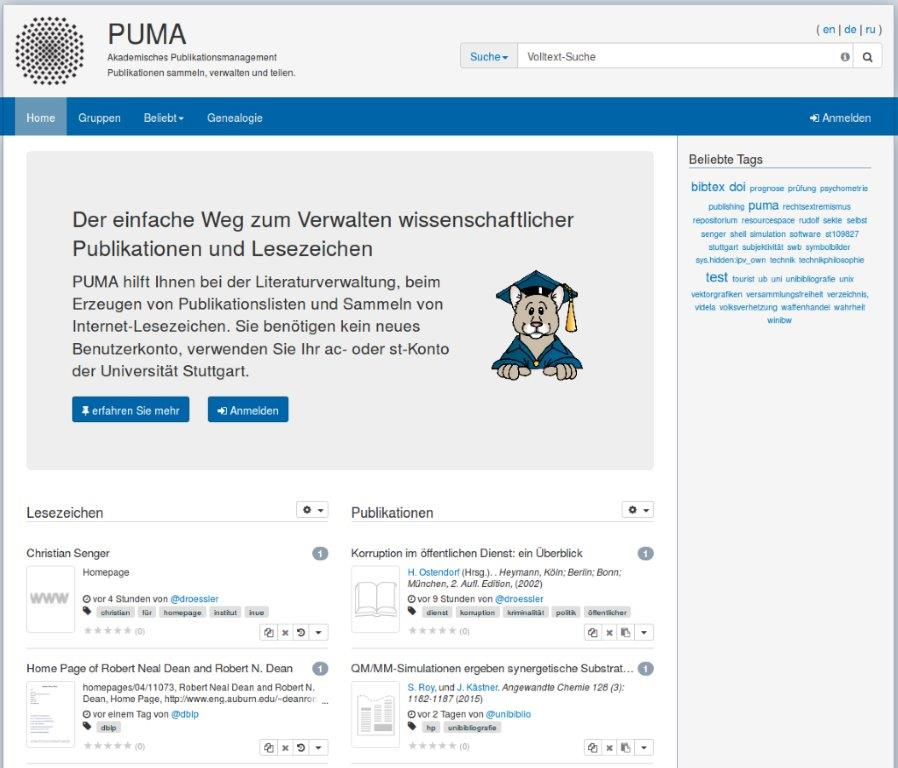
\includegraphics[scale=0.25]{puma-001.png}
 \caption{Startseite PUMA}
 \label{figure1}
\end{figure}

\textbf{Vorab:} Sie benötigen einen gültigen Bibliotheksausweis oder ein st-, fn- oder ac-Konto der Universität Stuttgart.
\begin{enumerate}
    \item Rufen Sie die Anmeldeseite von PUMA auf:\newline \url{https://puma.ub.uni-stuttgart.de/}
    \item Geben Sie unter \enquote{Benutzername} Ihr ac- oder st-Konto der Universität Stuttgart ein. Diesen finden Sie auf der Rückseite Ihres Bibliotheksausweises unterhalb des Strichcodes. %stimmt das?
    \item Unter  \enquote{Passwort} geben Sie Ihren Pin-Code ein. Bei der Ausstellung Ihres Ausweises wird dieser automatisch aus Ihrem Geburtsdatum generiert. Er hat das folgende Format: DDMMYY (DD= Tag (ggf. mit führender 0) / MM= Monat (ggf. mit führender 0) / YY= Jahr (die letzten zwei Ziffern des Geburtsjahres)). Beispiel: Wenn Sie am 25.03.1996 geboren sind, dann lautet Ihr Passwort: 250396.
 \begin{figure}[ht]
 \centering
 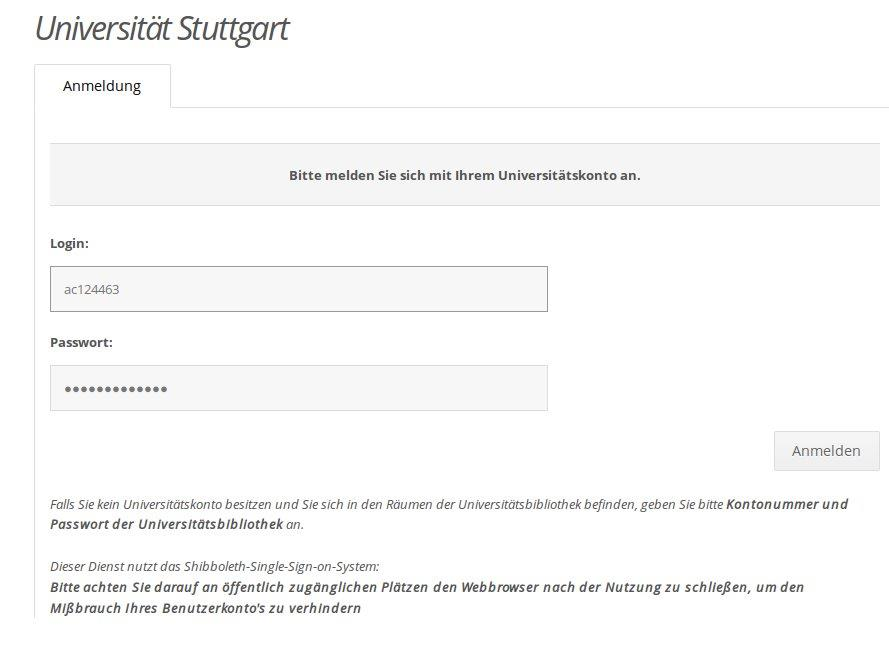
\includegraphics[scale=0.25]{puma-002.png}
 \caption{Anmeldung bei PUMA}
 \label{figure2}
\end{figure}  
    \item Klicken Sie auf \enquote{Anmelden}.
    \item Wenn Ihre Anmeldung erfolgreich war, dann zeigt Ihnen PUMA Ihre persönlichen Daten an (diese wurden bereits bei der Beantragung des Bibliotheksausweises hinterlegt). Überprüfen Sie die vorliegenden Daten und klicken Sie anschließend auf \enquote{Registrieren}.
\end{enumerate}
Die Anmeldung bei PUMA war erfolgreich. Ab sofort können Sie sich bei PUMA mit den Daten Ihres Bibliotheksausweises anmelden. \newline
Bei der erstmaligen Anmeldung ist die Vergabe eines Benutzernamens erforderlich. Bei öffentlich geteilten Einträgen erscheint er bei den Publiaktionseinträgen in der Form @benutzername.
\subsection{Der PUMA-Blog}


URL: http://blog.ub.uni-stuttgart.de/category/puma/
und RSS-Feed: http://blog.ub.uni-stuttgart.de/category/puma/feed/
(können die Nutzer für Infos zu Server-Updates abonnieren, vielleicht
kurze Anleitung für den Firefox dazu)
\subsection{BibSonomy\index{BibSonomy}}
PUMA steht nur den Mitgliedern der Universität Stuttgart zu Verfügung, die über ein st- oder ac-Konto  verfügen. Für externe Nutzer der Universitätsbibliothek Stuttgart besteht die Möglichkeit das Muttersystem von PUMA, BibSonomy, zu nutzen. Beide Systeme verfügen über die gleichen Funktionen und Möglichkeiten seine Publikationen und Lesezeichen zu sammeln, verwalten und teilen. \newline
Die Anmeldung bei BibSonomy erfolgt über die Homepage \url{http://www.bibsonomy.org/?lang=de}. 

\subsection{BibSonomy\index{BibSonomy} vs. PUMA}
\small
\begin{longtable}{|c|m{4cm}|m{4cm}|}\hline
	\bfseries Unterschiede & \bfseries PUMA & \bfseries BibSonomy\\ \hline
	Anmeldung& Nur möglich mit einem st-,fn- oder ac-Konto der Universität, mit dem sich die Nutzer authentifiziert  & Für jeden frei zugänglich, ein Benutzerkonto muss selber angelegt werden \\ \hline
	 Gruppen\index{Gruppen} & Gruppen können jederzeit und selbständig gegründet werden. & Die Gründung einer Gruppe erfordert die Freigabe des BibSonomy-Admins. \\ \hline
	OPUS\index{OPUS} & Für die Zukunft geplant. Ermöglicht den Nutzern ein direktes Veröffentlichen auf OPUS. & \\ \hline
	Unibibliografie\index{Unibibliografie}& Die Publikationsmetadaten der Unibibliografie stehen zum Beispiel für Institutspublikationslisten zur Nachnutzung zur Verfügung.&\\ \hline
\end{longtable}
\normalsize
